%\begin{figure*}[t]
%\centering
%\vspace{-2mm}
% 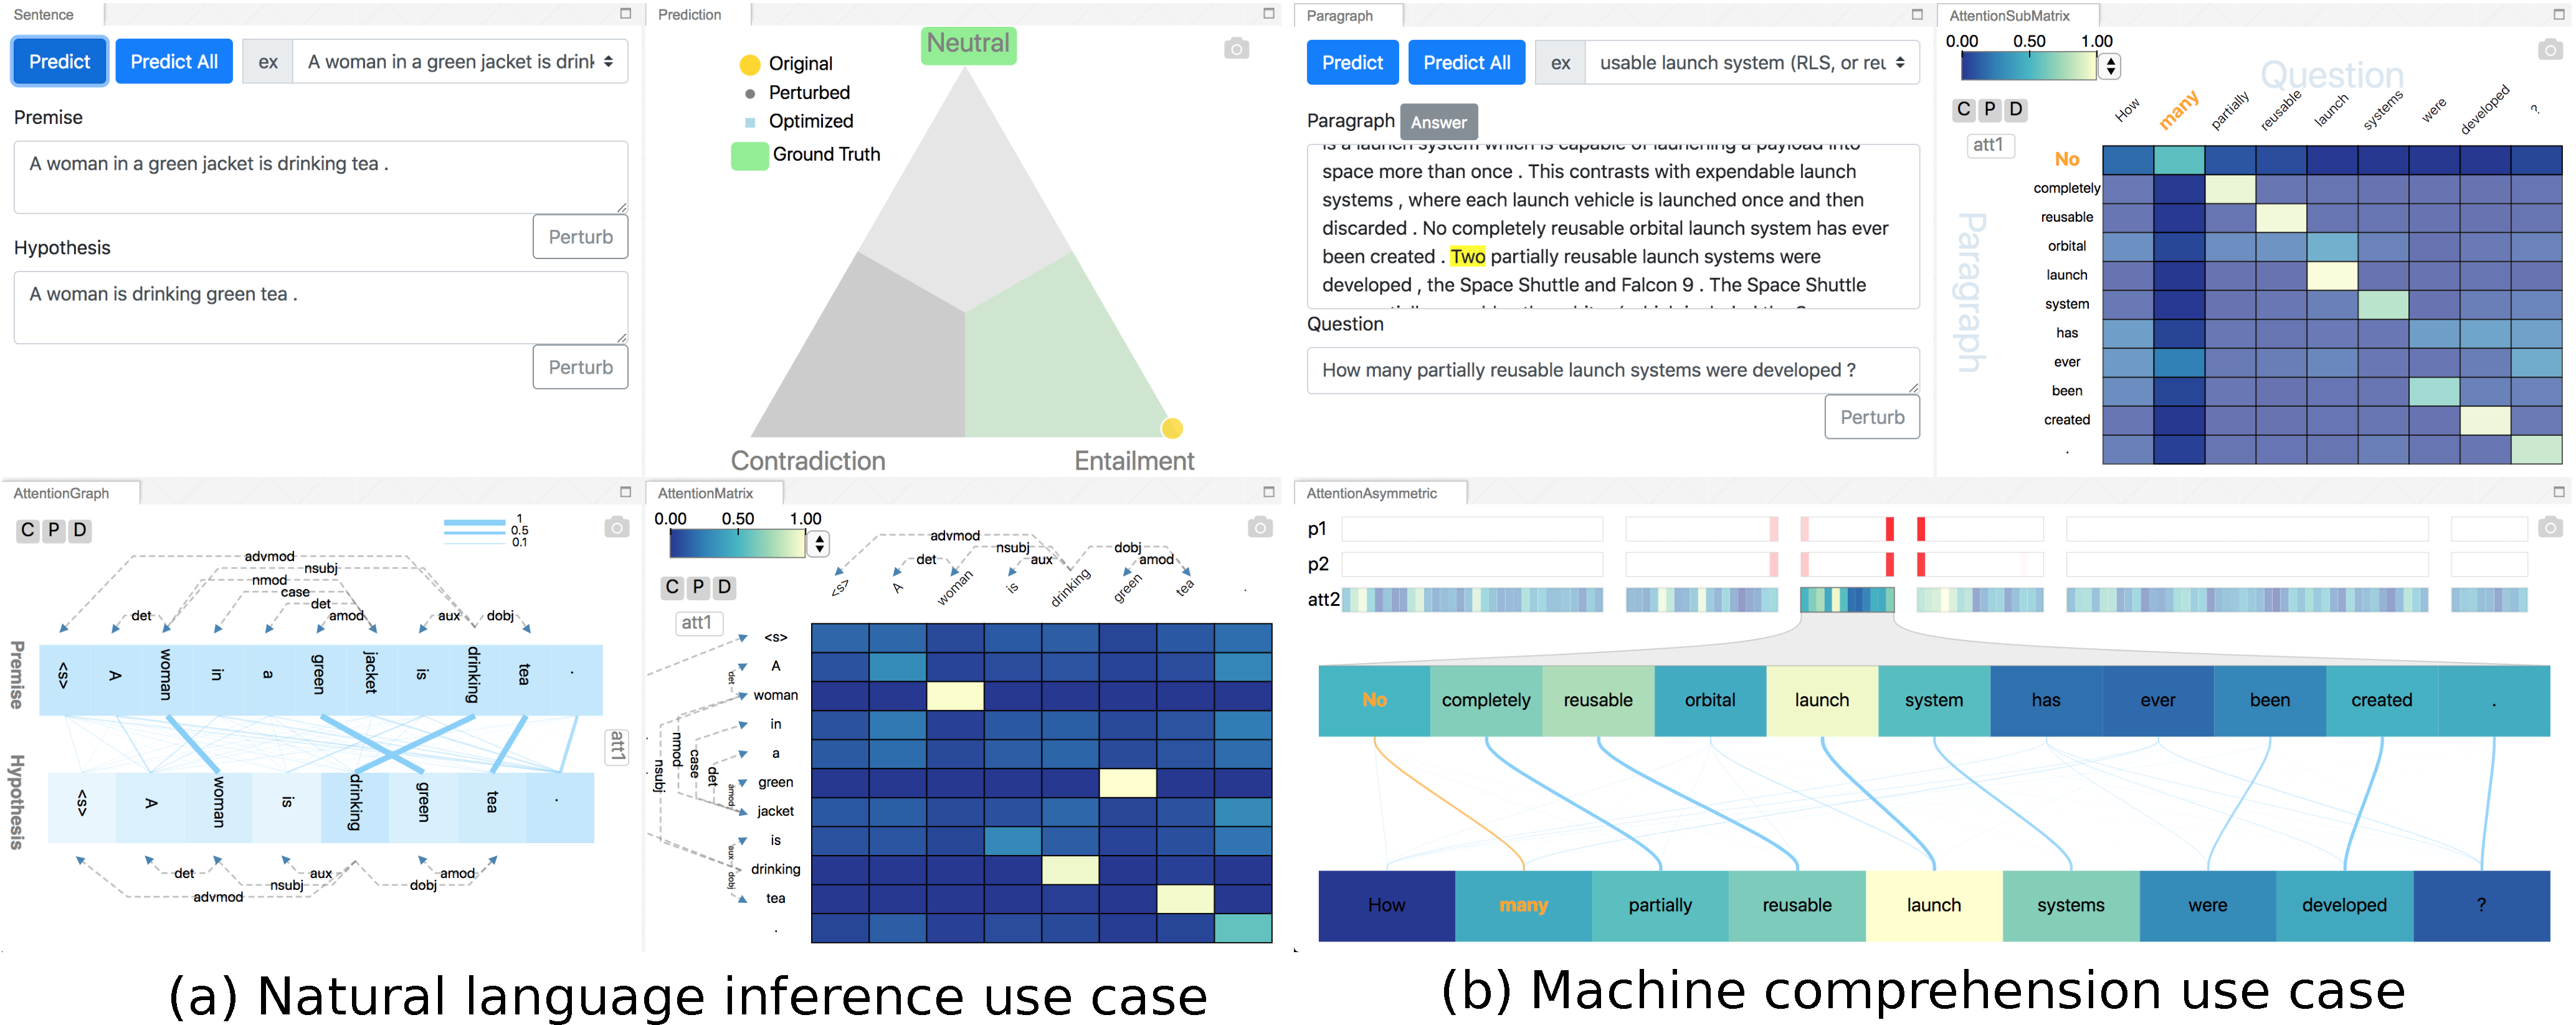
\includegraphics[width=1.0\linewidth]{NLI_MC_interface}
%  \vspace{-6mm}
% \caption{
%Illustration of different configurations for the natural language inference and machine comprehension tasks.
%}
%\label{fig:pipelineUpdate}
%\end{figure*}
\section{Applications}
We demonstrate the proposed visualization system on the decomposable attention network~\cite{parikh2016emnlp}
for the NLI task and the bi-directional attention flow network~\cite{Seo2016} for the MC task.

\begin{figure*}[t]
\centering
\vspace{-2mm}
 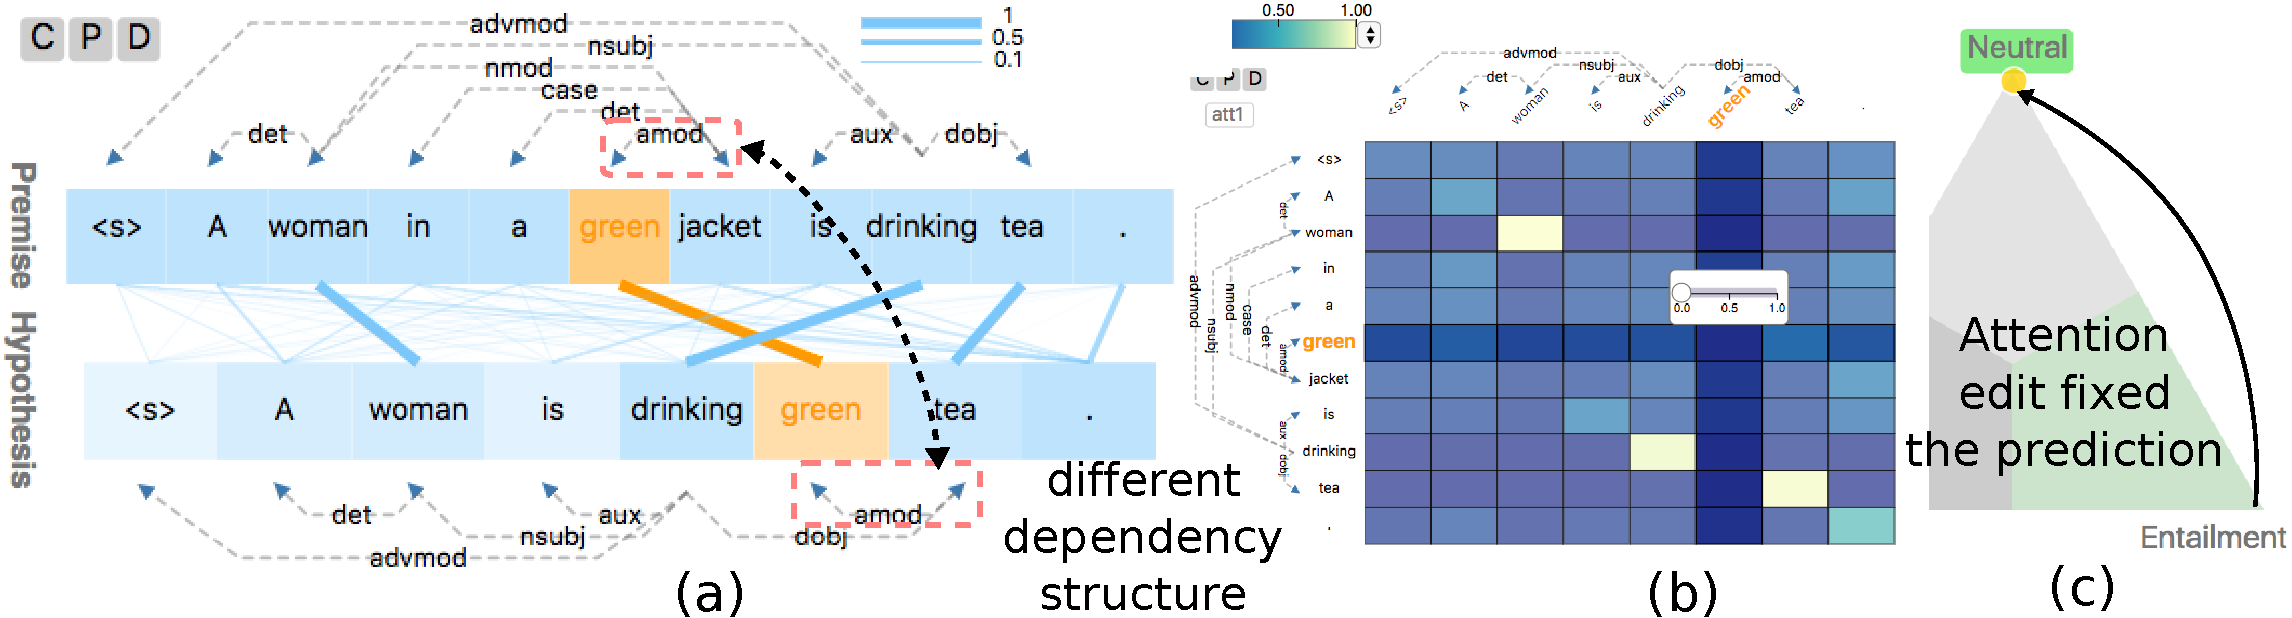
\includegraphics[width=1.0\linewidth]{NLIexample}
  \vspace{-6mm}
 \caption{
An illustrate of the attention editing process. 
By removing the alignment mistake between the two "green", the originally wrong prediction \emph{entailment} is corrected to \emph{netural}.
}
\label{fig:NLIexample}
\end{figure*}

\subsection{Natural Language Inference}
\label{sec:NLIexample}
The NLI task predict the relationship between a premise sentence (\textbf{P}) and a hypothesis sentence (\textbf{H}).
%as either \emph{entailment}, \emph{contradiction}, or \emph{neutral}.
%The model can be formalized as the following:
%%\begin{align}
%	$P^\prime, H^\prime = f(P), f(H)$,
%	$\overleftarrow{A} = P^\prime \cdot H^\prime$,
%	$\overrightarrow{A} = H^\prime \cdot P^\prime$,
%	$y = g(P, H, P^\prime, H^\prime, \overleftarrow{A}, \overrightarrow{A})$,
%%\end{align}
%where $P$ and $H$ are input embedding matrices for the premise and the hypothesis, $\overleftarrow{A}$
%and $\overrightarrow{A}$ are attentions, and $y$ is the predicted probabilities for candidate classes.
%Our system visualized the bidirectional attentions and their interaction with output distribution over labels.
The model produces two attention matrices, representing alignment from premise to hypothesis, and from hypothesis to premise.

Here we show an example, in which the wrong prediction can be fixed by correcting the attention value.  
%In the proposed system, we overlay the sentence dependency tree with the attention, which enables researchers to conduct comparisons between attention and grammar structure.
%
As illustrated in Fig.~\ref{fig:NLIexample}(a), the input sentence pairs (\textbf{P}:``A woman in a green jacket is drinking tea.'' \textbf{H}:``A woman is drinking green tea.'') is predicted to be entailment, which is incorrect.
By examining the attention, we can see the word \textbf{green} in ``\textbf{green} jacket" is aligned to the \textbf{green} in ``\textbf{green} tea", yet these two ``green'' decorate different nouns. Such a relationship can be confirmed by examining the dependency tree, where  \textbf{green} in \textbf{P} is attached to ``jacket'', whereas \textbf{green} in \textbf{H} is attached to ``tea''. However, the model does not aware of these the grammar information. As a result, the model mistakenly believes the two \textbf{greens} are used to describe the same thing (thus predict \emph{entailment}). 
%
To correct the mistake, we edit the attention value and remove the align between these two "green" (see Figure~\ref{fig:NLIexample}(b)).
As expected, the prediction label is corrected (\emph{neutral}) (see in Figure~\ref{fig:NLIexample}(c)).

\begin{figure*}[t]
\centering
\vspace{-2mm}
 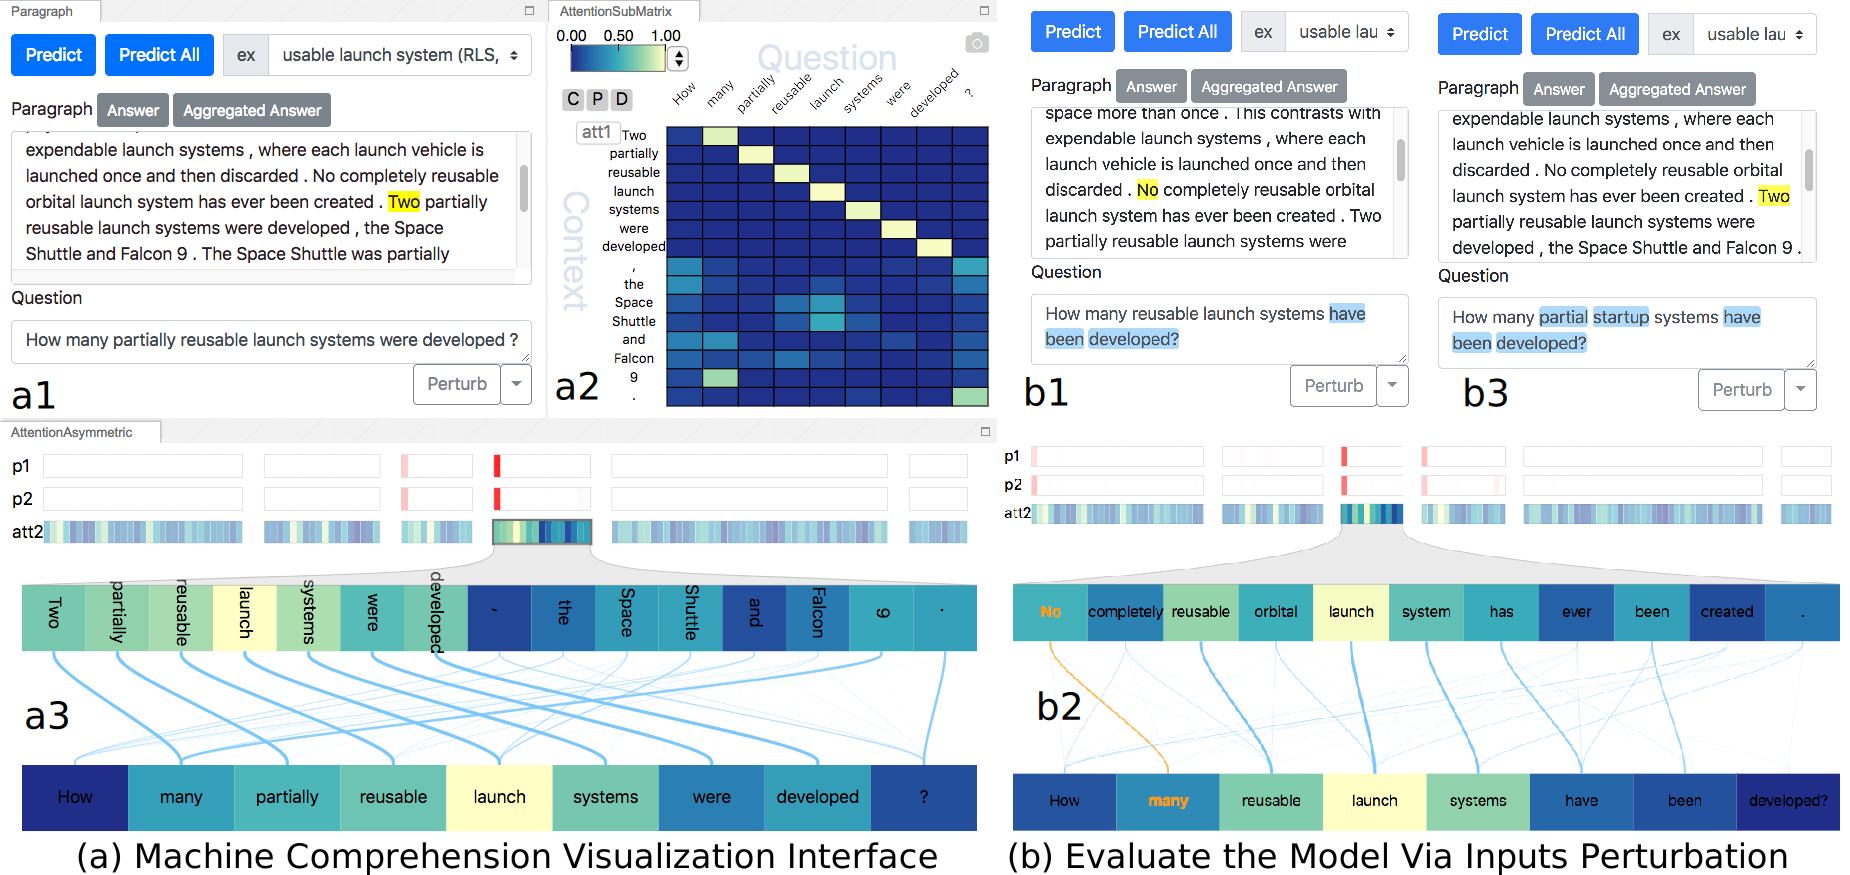
\includegraphics[width=1.0\linewidth]{MC_interface}
  \vspace{-6mm}
 \caption{
The proposed visualization help reveal the potential alignment issues in the machine comprehension model.
The $p1$, $p2$ color bar illustrate the predicted start and end index for the answer (deeper the red the higher the probability).
The answer to the question is found in (a1), where the ``Two'' is aligned with the ``many'' in the question. However, the number 9 is also aligned with many, which may potentially lead to confusions.
The second best answer is illustrated in b2.
}
\label{fig:MCexample}
\end{figure*}

\subsection{Machine Comprehension}
\label{sec:MCexample}
In machine comprehension task, two sequences of texts are given: context/paragraph and question.
The goal is to select a span of text from the context that answers the question. 
%We provide a simple model formulation and refer the reader to the paper for details.
%%\begin{align}
%	$C^\prime, Q^\prime = BiLSTM(C), BiLSTM(Q)$,
%	$\overleftarrow{A} = u(C^\prime, Q^\prime)$,
%	$\overrightarrow{A} = v(C^\prime, Q^\prime)$,
%	$s = m(C^\prime, Q^\prime, \overleftarrow{A}, \overrightarrow{A})$,
%	$e = n(s, C^\prime, Q^\prime, \overleftarrow{A}, \overrightarrow{A})$,
%%\end{align}
%where $C$ and $Q$ are embedding matrices for the context and the question,
%$\overleftarrow{A}$ and $\overrightarrow{A}$ are bidirectional attention flows,
%$s$ and $e$ are probabilities for starting and ending indices of the answer span.
%Our system reveals the internal states of $\overleftarrow{A}$, $\overrightarrow{A}$,
%$s$ and $e$.
Similarly, the attention information is also encoded as a bi-directional alignment (i.e., from context to question and vice versa). 
The key difference is how the question to context alignment is computed (see \cite{Seo2016} for more details).
Here, we refer the context to question attention as \emph{att1}, and question to context attention as \emph{att2}.

As illustrated in Figure~\ref{fig:MCexample}, we show \emph{att2} in the overview attention colored bars (yellow-green-blue colormap), in which each rectangular corresponds to one sentence. We can then focus on individual sentences by click on the rectangular (see Figure~\ref{fig:MCexample}).
%The proposed visualization help reveal the potential alignment issues in the machine comprehension model.
The $p1$, $p2$ colored bars (white-red colormap) illustrate the predicted start and end index for the answer (deeper the red the higher the probability). The span of text defined by the start and end index with the highest probability is the answer.
%
As we can see, there are two spans of text that correspond to higher probabilities. We can examine the corresponding sentence in (a3) and (b2). Both sentences exhibit excellent alignment with the question. The spans with high probability are ``Two'' and ``No'' (highlight in orange), which both align well with many.
Another interesting observation is that the number ``9'' (in ``Falcon 9') is also aligned with ``many'', yet in the prediction both ``Two'' and ``No'' have significantly higher probability.
One possible explanation is the word ``Two'' has much higher \emph{att2} attention value compare to ``9'', which may contribute to the current outcome.
